%\pdfminorversion=4 % needed to be able to print it for some reason
\documentclass[a0paper,portrait,twocols]{def/LiUposter} % there is also A1, but work with A0 and print on A1

\usepackage{def/myposter}



\title{\Huge{\bfseries Track Fusion Design in Decentralized Target Tracking} } % \vspace{0.5em} \\ \huge{{A Minimal Set of Evaluation Measures}}
\author{Robin Forsling [\texttt{robin.forsling@liu.se}]} 
\institute{Division of Automatic Control} % Department of Electrical Engineering



% BEGIN POSTER
\begin{document}


% TOP ROW
%\vspace{-5cm}
%{\begin{minipage}[t][1.98\columnwidth][s]{1.98\columnwidth}
%
%\begin{mycolumnbox}[width=2.05\columnwidth,height=20cm]
%\end{mycolumnbox}
%\end{minipage}} 





% LEFT COLUMN
{\begin{minipage}{\columnwidth} 


\vspace{-3em}




% SUMMARY

\begin{mybox}[title={Summary}]{mydarkgreen}
The \textbf{design of a track fusion} subsystem in a decentralized single-target tracking (DSTT) system is considered. The approach is to evaluate different track fusion methods using two measures: \textbf{RMT}, related to \emph{tracking performance}; and \textbf{COIN}, related to \emph{uncertainty assessment}.
\end{mybox}




% BACKGROUND
\subsection{Background}

\begin{center}
	\begin{tikzpicture}[scale=.9]
		
% AGENTS
\def\ra{0.75}




% --- FIGURE ---
\BFS

\drawtargettrajectory [path fading=east] plot [smooth, tension=1] coordinates {(0,0) (7,5) (15,1) (24,3) (30,4)};
\node at (0,0) {\mycircle{black}};


% AGENT 1
\def\xa{(-8,3)}
\draw [rotate around={-20:\xa}] \sensoropt{clra} \xa -- (-3,5) to [out=-60,in=60] (-3,1) -- cycle;	
\drawcomarrow[->,rotate around={11:\xa}] \xa -- (-4,3);
\drawagent{clra} \xa circle [radius = \ra];


% AGENT 2
\def\xa{(15,8)}
\draw [rotate around={-140:\xa}] \sensoropt{clrb} \xa -- (20,10) to [out=-60,in=60] (20,6) -- cycle;
\drawcomarrow[->,rotate around={11:\xa}] \xa -- (11,8);
\drawcomarrow[->,rotate around={-35:\xa}] \xa -- (19,8);
\drawagent{clrb} \xa circle [radius = \ra];


% AGENT 3
\def\xa{(27,0)}
\draw [rotate around={180:\xa}] \sensoropt{clrc} \xa -- (32,2) to [out=-60,in=60] (32,-2) -- cycle;	
\drawcomarrow[->,rotate around={-35:\xa}] \xa -- (23,0);
\drawagent{clrc} \xa circle [radius = \ra];


\EFS
	\end{tikzpicture}	
\end{center}

Consider the DSTT scenario above. Multiple agents (colored circles) use sensor measurements to estimate the state of a common dynamic target (black circle). The track estimates are communicated between the agents for fusion. Tracking a common target implies correlations between local track estimates. The main sources of correlations are:
\begin{itemize}
	\item \emph{Common process noise}. Correlations that appear since the same process (target) is tracked by the different agents.
	\item \emph{Common information}. Correlations that appear due to the sharing and fusion of information. 
\end{itemize} 
If these correlations are not handled properly, the track uncertainties will be \emph{\textcolor{myorange}{underestimated}} which means that the tracks \emph{\textcolor{myorange}{cannot be trusted}}.




% TARGET MODEL
%\subsection{Target Model}

%\begin{mybox}[title={Target State-Space Model}]{darkgray}
%Let $x_k$ be the target state at time $k$. The following linear state-space model is assumed:
%\begin{align*}
%	x_{k+1} &= F_kx_k + w_k, & w_k &\sim \calN(0,Q_k), \\
%	z_k &= H_kx_k + e_k, & e_k &\sim \calN(0,C_k),
%\end{align*}
%where $F_k$ is the state transition model, $Q_k$ is the process noise covariance, $z_k$ is a measurement, $H_k$ is the measurement model, and $C_k$ is the measurement noise covariance, at time $k$. 
%\end{mybox}






% DSTT SYSTEM
\subsection{A Decentralized Single-Target Tracking System}

\vspace{0.5em}

\begin{center}
	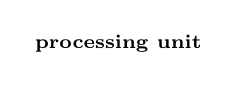
\begin{tikzpicture}[scale=3]
		
% --- FIGURE ---
\begin{scriptsize}

%\draw [white,opacity=.0] (0,-1) rectangle (17,0);

\drawprocessingunitbox{clra!40!} (2.75,-1.75) rectangle (9.75,2);
\node [below,font=\bfseries] at (6.25,2) {processing unit};

% STATE EST
\drawsensorbox (0,0) rectangle (2,1) node [pos=.5,font=\bfseries,color=white] {sensors};
\drawsystemarrow (2,0.5) -- (3,0.5);
\drawsystembox (3,0) rectangle (5.5,1) node [pos=.5,font=\bfseries,align=center] {state \\ estimation};
\drawsystemarrow (4.25,0) -- (4.25,-0.5);

% FUSION
\drawsensorbox (0,-0.5) rectangle (2,-1.5) node [pos=.5,font=\bfseries,align=center,color=white] {datalink};
\drawsystemarrow (2,-1) -- (3,-1);
\drawsystembox (3,-0.5) rectangle (5.5,-1.5) node [pos=.5,font=\bfseries,align=center] {track \\ fusion};

% COM
\drawsystemarrow (5.5,-1) -- (6.5,-1);
%\drawsystemarrow [densely dashed] (10.75,-1) -- (10.75,1.25) -- (5,1.25) -- (5,1);
%\draw [black,fill=black] (10.75,-1) circle [radius=0.05];
\drawsystembox (6.5,-0.5) rectangle (9.5,-1.5) node [pos=.5,font=\bfseries,align=center] {communication \\ management};
\drawsystemarrow (9.5,-1) -- (10.5,-1) node [near start,above right,align=center,font=\it] {exchanged \\ track};

\end{scriptsize}
	\end{tikzpicture}
\end{center}

A DSTT system is illustrated above. It contains three main components:
\begin{enumerate}
	\item \emph{State estimation}. Predicts and updates the target state estimate using local sensor measurements.
	\item \emph{Track fusion}. Fuses the received tracks with the local track.
	\item \emph{Communication management}. Handles what, when, and with whom to communicate.
\end{enumerate}
The state estimation is solved using a Kalman filter. The communication management is given. %The track fusion is to be designed by evaluating different track fusion methods as follows.




\begin{mybox}[title={Problem}]{mydarkgreen}
Design the \emph{track fusion} such that sufficient track quality is obtained. In particular, the track fusion design must consider two aspects:
\begin{itemize}
	\item Sufficient tracking performance in terms of the tracking error.
	\item Credible (trustworthy) assessment of the track uncertainty.
\end{itemize}
\end{mybox}
The credibility criterion is introduced to quantify if the track uncertainty is underestimated or not.



% TARGET MODEL
\subsection{Notation}

Let $x_k$ be the target state at time $k$. An estimate of $x_k$ at time $k$ is given by $(\xhat_k,P_k)$, where $\xhat_k$ is the state estimate and $P_k$ is the computed covariance. The track fusion design is evaluated using Monte Carlo (MC) simulations, with $M$ denoting the number of MC runs. An estimate $(\xhat_k,P_k)$ in the \ith MC run is denoted $(\xhat_k^i,P_k^i)$. The estimation error is denoted $\xtilde_k=\xhat_k-x_k$ or $\xtilde_k^i=\xhat_k^i-x_k$.




\end{minipage} % END LEFT COLUMN





      
% RIGHT COLUMN    
\begin{minipage}{\columnwidth}


\vspace{-3em}



% RMT
\subsection{RMT: A Tracking Performance Measure}

Tracking performance is often evaluated using the root mean squared error (RMSE). However, since RMSE requires the true error to be known, RMSE cannot be computed online. What a user has access to is $P_k$. Hence, the \emph{root mean trace} (RMT) is used instead:
\begin{equation*}
	\boxed{\text{RMT}_k = \sqrt{\trace\left(\frac{1}{M}\sum_{i=1}^M P_k^i\right)} = \sqrt{\frac{1}{M}\sum_{i=1}^M \trace(P_k^i)}}
\end{equation*}
A smaller RMT is interpreted as better tracking performance.
 



% COIN
\subsection{COIN: An Uncertainty Assessment Measure}

To quantify the uncertainty assessment, the notion of conservativeness is used. An estimate $(\xhat_k,P_k)$ is \emph{conservative} if
\begin{equation}
	P_k - \EV(\xtilde_k\xtilde_k\trnsp) = P_k - \Ptilde_k \succeq 0,
	\label{eq:conservative-estimate}
\end{equation}
where $\Ptilde_k-\EV(\xtilde_k\xtilde_k\trnsp)$. Let $P_k=L_kL_k\trnsp$. Then the condition in \eqref{eq:conservative-estimate} is equivalent to $I\succeq L_k\inv\Ptilde_k L_k\invtrnsp$. Let $\lambdamax(\cdot)$ denote the largest eigenvalue. The \emph{conservativeness index} (COIN) is defined as:
\begin{equation*}
	\boxed{\text{COIN}_k = \lambdamax\left(L_k\inv\Ptilde_k L_k\invtrnsp\right)}
\end{equation*} 
An estimate is conservative \textiff COIN$_k\leq 1$. If $\Ptilde_k$ is unknown it can be approximated by
\begin{equation*}
	\Phat_k = \frac{1}{M} \sum_{i=1}^M \xtilde_k^i(\xtilde_k^i)\trnsp.
\end{equation*} 




% EVALUATION
\subsection{Design Evaluation}

The design evaluation is illustrated using a DSTT scenario with three agents. For more information about the evaluation scenario, see:
 
\begin{center}
	\url{https://github.com/robinforsling/dtt}
\end{center}

The evaluated track fusion methods are: covariance intersection (CI); inverse covariance intersection (ICI); the largest ellipsoid (LE) method; and the \naive Kalman fuser (NKF).

%\vspace{1em}


\begin{mybox}[title={Design Evaluation Results}]{darkgray}
\begin{center}
	\begin{tikzpicture}[xscale=1.15]
		
\newcommand*\drawkf{\draw[line width=2mm,clrkf]}
\newcommand*\drawci{\draw[line width=2mm,clrci]}
\newcommand*\drawici{\draw[line width=2mm,clrici]}
\newcommand*\drawle{\draw[line width=2mm,clrle]}
\newcommand*\plotcommand{plot[smooth]coordinates}

\def\ks{1}
\def\kend{12}

\def\xleg{0}
\def\yleg{19}
\def\lleg{1.25}
\def\sleg{8}

\def\addaneesconfidence{\drawaneesconfidence(\ks,.9811)rectangle(\kend,1.0191);}




% --- FIGURE ---
%\BFS




% RMT
\def\addxlabel{\node at (6.5,2.0) {$k$};}
\def\addylabel(#1){\node[rotate=90] at (-2,9) {#1};}
\def\ymin{4}; \def\ymax{14}

\begin{scope}[yscale=1.2]
	
\drawkf\plotcommand{(2,8.129)(5,5.165)(8,4.832)(11,4.820)};
\drawci\plotcommand{(2,12.713)(5,8.395)(8,7.912)(11,7.893)};
\drawici\plotcommand{(2,11.812)(5,7.640)(8,7.359)(11,7.356)};
\drawle\plotcommand{(2,10.770)(5,6.969)(8,6.747)(11,6.743)};
\foreach \y in {6,8,...,12} {\drawytick(\ks,\y);\node [left] at (\ks,\y) {\y};}
\foreach \x in {2,5,...,11} {\drawxtick(\x,\ymin);\node [below] at (\x,\ymin) {\x};}
\drawcoordinateframe(\ks,\ymax)--(\ks,\ymin)--(\kend,\ymin);	
\addylabel(RMT)
\addxlabel
	
\end{scope}




% COIN
\def\addxlabel{\node at (6.5,0.1) {$k$};}
\def\addylabel(#1){\node[rotate=90] at (-2,1.5) {#1};}
\def\ymin{0.5}; \def\ymax{2.5}

\begin{scope}[xshift=16cm,yshift=1.65cm,yscale=6]

\drawsupportline(\ks,1)--(\kend,1);
\drawkf\plotcommand{(2,2.068)(5,2.224)(8,2.300)(11,2.419)};
\drawci\plotcommand{(2,0.734)(5,0.841)(8,0.904)(11,0.892)};
\drawici\plotcommand{(2,0.796)(5,0.904)(8,0.922)(11,0.909)};
\drawle\plotcommand{(2,1.076)(5,1.125)(8,1.093)(11,1.068)};
\foreach \y in {1.0,1.5,2.0} {\drawytick(\ks,\y);\node [left] at (\ks,\y) {\y};}
\foreach \x in {2,5,...,11} {\drawxtick(\x,\ymin);\node [below] at (\x,\ymin) {\x};}
\drawcoordinateframe(\ks,\ymax)--(\ks,\ymin)--(\kend,\ymin);
\addylabel(COIN)
\addxlabel

\end{scope}




% LEGEND:

\drawci({\xleg},\yleg)--({\xleg+\lleg},\yleg) node [right,black] {CI};
\drawici({\xleg+\sleg},\yleg)--({\xleg+\lleg+\sleg},\yleg) node [right,black] {ICI};
\drawle({\xleg+2*\sleg},\yleg)--({\xleg+\lleg+2*\sleg},\yleg) node [right,black] {LE};
\drawkf({\xleg+3*\sleg},\yleg)--({\xleg+\lleg+3*\sleg},\yleg) node [right,black] {NKF};



%\EFS






	\end{tikzpicture}
\end{center}

%\paragraph{Observations}
NKF yields the best tracking performance but is clearly non-conservative due to poor uncertainty assessment. CI and ICI are conservative \wrt COIN. LE yields better tracking performance than CI and ICI, but the COIN values for LE are slightly above 1.

\paragraph{Concluding Remarks}
\begin{itemize}
	\item Choosing the most suitable track fusion method is a compromise between tracking performance and uncertainty assessment.
	\item Ultimately, the selected track fusion method must provide satisfactory results and tracking quality to the end user.
\end{itemize}

\end{mybox}



\end{minipage}} % END RIGHT COLUMN



    

 	 
\end{document}


